\documentclass[preview, border=15pt]{standalone}
\usepackage{mathtools, commath}
% Packages for formatting
\usepackage[margin=1in]{geometry}
\usepackage{fancyhdr}
\usepackage{enumerate}
\usepackage{graphicx}
\usepackage{kotex}
\usepackage{arydshln} % Include this package
\usepackage{bbding}
\usepackage{amsmath}
\usepackage{amsthm}
\usepackage[dvipsnames,table]{xcolor}
\usepackage{amssymb, amsfonts}
\usepackage{wasysym}
\usepackage{footnote}
\usepackage{tablefootnote}
\usepackage{arydshln} % Include this package

% Fonts
\usepackage[T1]{fontenc}
\usepackage[utf8]{inputenc}
\usepackage{newpxtext,newpxmath}
\usepackage{sectsty}

\usepackage{animate}
% Load the PDF and grab its total pages into \NumPages:
\newcount\NumPages
\pdfximage{../riemann-tikz/cycloid_gif.pdf}% loads the PDF
\NumPages=\pdflastximagepages

\begin{document}
\begin{center}
	\animateinline[autoplay,loop]{5}% 5 fps
	\multiframe{\the\NumPages}{i=1+1}{%
		\includegraphics[page=\i,width=0.75\linewidth]{../riemann-tikz/cycloid_gif.pdf}%
	}
	\endanimateinline
\end{center}

\begin{center}
	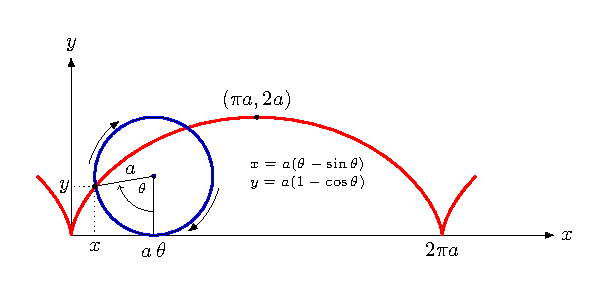
\includegraphics[scale=1.25]{../riemann-tikz/cycloid}
\end{center}
Let 
\[
\mathbf r(t)
=\bigl\langle x(t),\,y(t)\bigr\rangle
=\bigl\langle R\,t - R\sin t,\;R - R\cos t\bigr\rangle,
\quad t\in[0,2\pi].
\]
Then
\[
\mathbf r'(t)
=\bigl\langle x'(t),\,y'(t)\bigr\rangle
=\bigl\langle R(1-\cos t),\;R\sin t\bigr\rangle.
\]
The differential arc–length is
\[
\bigl\|\mathbf r'(t)\bigr\|\,dt
=\sqrt{\bigl[R(1-\cos t)\bigr]^2 + \bigl[R\sin t\bigr]^2}\;dt.
\]
Inside the square‐root:
\[
R^2(1-\cos t)^2 + R^2\sin^2t
=R^2\bigl[1 -2\cos t+\cos^2t +\sin^2t\bigr]
=R^2\bigl[2 -2\cos t\bigr]
=2R^2\bigl(1-\cos t\bigr).
\]
Hence
\[
\|\mathbf r'(t)\|
=\sqrt{2R^2(1-\cos t)}
=R\sqrt{2(1-\cos t)}
=2R\bigl|\sin\!\tfrac t2\bigr|.
\]
On \(0\le t\le2\pi\), \(\sin(t/2)\ge0\), so
\[
\|\mathbf r'(t)\|=2R\sin\!\tfrac t2.
\]
The total length of one arch is
\[
L=\int_0^{2\pi}\|\mathbf r'(t)\|\,dt
=\int_0^{2\pi}2R\sin\!\tfrac t2\;dt.
\]
Make the substitution \(u=\tfrac t2\), so \(dt=2\,du\) and when \(t\) runs from \(0\) to \(2\pi\), \(u\) runs from \(0\) to \(\pi\):
\[
L
=2R\int_{0}^{2\pi}\sin\!\tfrac t2\,dt
=2R\int_{0}^{\pi}\sin u\,(2\,du)
=4R\int_{0}^{\pi}\sin u\,du
=4R\bigl[-\cos u\bigr]_0^{\pi}
=4R\bigl[-(-1)-(-1)\bigr]
=8R.
\]
\[
\boxed{L_{\mathrm{one\;arch}}=8R.}
\]
\end{document}